\let\negmedspace\undefined
\let\negthickspace\undefined
\documentclass[journal,12pt,onecolumn]{IEEEtran}
\usepackage{cite}
\usepackage{amsmath,amssymb,amsfonts,amsthm}
\usepackage{algorithmic}
\usepackage{graphicx}
\graphicspath{{./figs/}}
\usepackage{textcomp}
\usepackage{xcolor}
\usepackage{txfonts}
\usepackage{listings}
\usepackage{enumitem}
\usepackage{mathtools}
\usepackage{gensymb}
\usepackage{comment}
\usepackage{caption}
\usepackage[breaklinks=true]{hyperref}
\usepackage{tkz-euclide} 
\usepackage{listings}
\usepackage{gvv}                                        
%\def\inputGnumericTable{}                                 
\usepackage[latin1]{inputenc}     
\usepackage{xparse}
\usepackage{color}                                            
\usepackage{array}
\usepackage{longtable}                                       
\usepackage{calc}                                             
\usepackage{multirow}
\usepackage{multicol}
\usepackage{hhline}                                           
\usepackage{ifthen}                                           
\usepackage{lscape}
\usepackage{tabularx}
\usepackage{array}
\usepackage{float}
\usepackage{parskip}
\newtheorem{theorem}{Theorem}[section]
\newtheorem{problem}{Problem}
\newtheorem{proposition}{Proposition}[section]
\newtheorem{lemma}{Lemma}[section]
\newtheorem{corollary}[theorem]{Corollary}
\newtheorem{example}{Example}[section]
\newtheorem{definition}[problem]{Definition}
\newcommand{\BEQA}{\begin{eqnarray}}
\newcommand{\EEQA}{\end{eqnarray}}
\newcommand{\define}{\stackrel{\triangle}{=}}
\theoremstyle{remark}
\newtheorem{rem}{Remark}

\begin{document}
\title{4.7.42}
\author{EE25BTECH11045 - P.Navya Priya}
\maketitle
\renewcommand{\thefigure}{\theenumi}
\renewcommand{\thetable}{\theenumi}
\textbf{Question:}

Find the length and the foot of perpendicular from the point $\brak{1,\frac{3}{2},2}$ to the plane $2\text{x}-2\text{y}+4\text{z}+5=0$.

\textbf{Solution:}

Given plane equation $2\text{x}-2\text{y}+4\text{z}+5=0$ can be written as 
\begin{align}
    \vec{n}^\top\vec{x}=c
\end{align}
Where
\begin{align*} 
    \vec{n}=\myvec{2\\-2\\4}\;\text{and}\;\text{c}=-5
\end{align*}
Let the point be $\vec{p}\myvec{1\\[3pt]\frac{3}{2}\\[3pt]2}$ and the point on the plane be $\vec{x_o}$. The equation of the line joining $\vec{p}$ and $\vec{x_o}$ is
\begin{align}
    \vec{x_o}\,=\,\vec{p}\,+\,\lambda\vec{n}
\end{align}
Multiply equation(2) on both sides by $\vec{n}^\top$
\begin{align}
\vec{n}^\top\brak{\vec{x_o}}\,=\,\vec{n}^\top\brak{\vec{p}\,+\,\lambda\vec{n}}
\end{align}
\begin{align}
\lambda\,=\,\frac{\vec{n}^\top\vec{x}_o}{\vec{n}^\top\vec{p}\,+\,\lambda\vec{n}^\top\vec{n}}
\end{align}
\begin{align}
    \lambda=\frac{-5}{\brak{2\,-2\,\,\,4}\myvec{1\\[3pt]\frac{3}{2}\\[3pt]2}\,+\,\lambda\brak{2\,-2\,\,\,4}\myvec{2\\-2\\4}}(\because \vec{n}^\top\vec{x_o}=-5)
\end{align}
\begin{align}
    \lambda\,=\,-\frac{1}{2}
\end{align}
Substitute the value of $\lambda$ in equation(2) to get $\vec{x}_o$
\begin{align}
    \vec{x}_o\,=\,\myvec{0\\[3pt]\frac{5}{2}\\[3pt]0}
\end{align}
\begin{align*}
    \therefore \textbf{Foot of perpendicular}\; \text{is}\; \vec{x}_o\,=\,\myvec{0\\[3pt]\frac{5}{2}\\[3pt]0}
    \end{align*}
\newpage
The length of point $\myvec{1\\[3pt]\frac{3}{2}\\[3pt]2}$ to the plane $2\text{x}-2\text{y}+4\text{z}+5=0$ is
\begin{align}
    ||\vec{x_o}-\vec{p}||\,&=\,\sqrt{\brak{\vec{x_o}-\vec{p}}^\top\brak{\vec{x_o}-\vec{p}}}\\
    &=\sqrt{6}
\end{align}
\begin{align*}
    \therefore ||\vec{x_o}-\vec{p}||\,=\,\sqrt{6}
\end{align*}

From the graph, theoretical solution matches with the computational solution.

\begin{figure}[H]
\centering
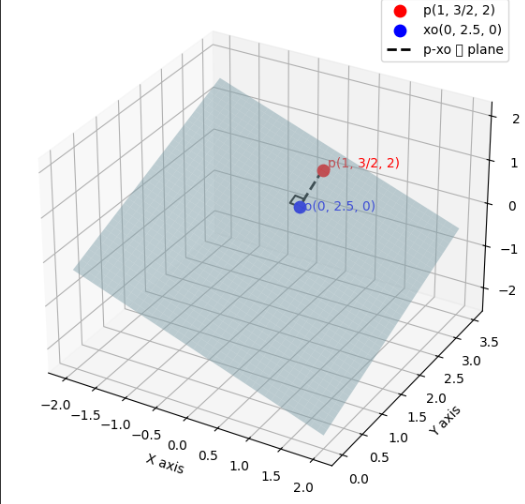
\includegraphics[width=0.7\columnwidth]{figs/graph.png}
\caption*{Perpendicular to the plane (length=$\sqrt{6}$)}
\label{fig:graph.png}
\end{figure}
\end{document}